\documentclass[11pt]{book}
\usepackage{gvv-book}
\usepackage{gvv}
\usepackage[sectionbib,authoryear]{natbib}
\setcounter{secnumdepth}{3}
\setcounter{tocdepth}{2}
\makeindex

\begin{document}
\frontmatter
\tableofcontents
\setcounter{page}{1}
\mainmatter
\chapter{Triangle}
Consider a triangle with vertices
\begin{align}
\label{eq:tri-pts}
\vec{A}=\myvec{1 \\ 0},\,
\vec{B}=\myvec{5\\4},\,
	\vec{c}=\myvec{-4\\0},\,
\end{align}

\section{Vectors}
\section{Median}
\section{Altitude}
\section{Perpendicular Bisector}
\section{Angular Bisector}
\section{Matrix}

The matrix of the veritices of the triangle is defined as
		\begin{align}
			\vec{P} &= \myvec{\vec{A} & \vec{B} &\vec{C}} \\
            &=\myvec{1 & 5 & -4 \\ 0 & 4 & 0}
		\end{align}
\begin{figure}[H]
    \centering
    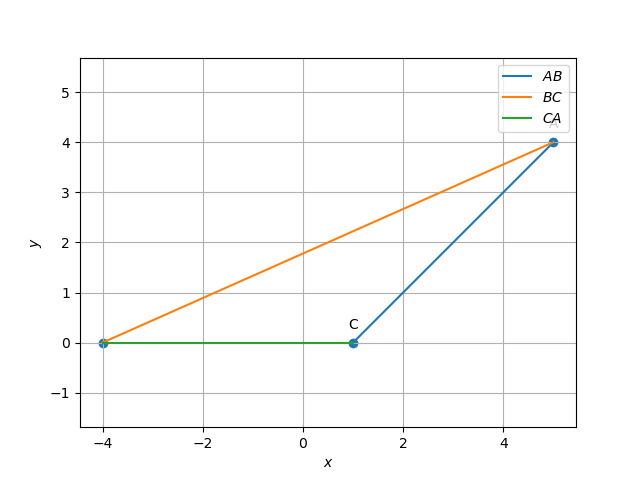
\includegraphics{/sdcard/digital-design/figs/ABC.png}
    \caption{$\triangle$ ABC}
    \label{fig:mat_vec1}
\end{figure}
\subsection{Vectors}


\begin{enumerate}[label=\thesubsection.\arabic*.,ref=\thesubsection.\theenumi]
\numberwithin{equation}{enumi}
%Question 1.6.1.1
\item Obtain the direction matrix of the sides of $\triangle ABC$ defined as 
\begin{align}
\vec{M} = 	\myvec{\vec{A}-\vec{B} & \vec{B}-\vec{C} & \vec{C}-\vec{A}}
\end{align}
\\
\solution 
\begin{align}
\vec{M} &= \myvec{\vec{A}-\vec{B} & \vec{B}-\vec{C} & \vec{C}-\vec{A}} \\
	&= \myvec{\vec{A} & \vec{B} &\vec{C}} \myvec{1 & 0 & -1 \\ -1 & 1 & 0 \\ 0 & -1 & 1} \\
 &=\myvec{1 & 5 & -4 \\ 0 & 4 & 0}\myvec{1 & 0 & -1 \\ -1 & 1 & 0 \\ 0 & -1 & 1} 
 \end{align}
 Using Matrix multiplication
 \begin{align}
 \vec{M} &=\myvec{-4 & 9 & -5 \\ -4 & 4 & 0}
\end{align}
where the second matrix above is known as a {\em circulant} matrix.  Note that the 2nd and 3rd row of the above matrix are circular shifts of the 1st row.
%Question 1.6.1.2
\item Obtain the normal matrix  of the sides of $\triangle ABC$ \\
\solution Considering the roation matrix
\begin{align}
\vec{R}  = \myvec{0 & -1 \\ 1 & 0},
\end{align}
the normal matrix is obtained as
\begin{align}
\vec{N} &= \vec{R}\vec{M}  \\
&=\myvec{0 & -1 \\ 1 & 0}\myvec{-4 & 9 & -5 \\ -4 & 4 & 0}
\end{align}
Using matrix multiplication 
\begin{align}
   \vec{N} &= \myvec{4 & -4 & 0 \\ -4 & 9 & -5}
\end{align}
%Question 1.6.1.3
\item Obtain $a, b, c$. \\
\solution The sides vector is obtained as
\begin{align}
\vec{d} &= \sqrt{\text{diag}(\vec{M}^{\top}\vec{M})}\\
\vec{M}^{\top}\vec{M} &= \myvec{4&-4 \\ -4 &9 \\ 0 &-5}\myvec{4 & -4 & 0 \\ -4 & 9 & -5}
\end{align} 
Using matrix multiplication 
\begin{align}
    \vec{M} &= \myvec{ 32 & -52 & 20 \\ -52 & 97 & -45 \\ -20 & 45 & -25} \\
    \vec{d} &= \sqrt{\text{diag}\brak{\myvec{ 32 & -52 & 20 \\ -52 & 97 & -45 \\ -20 & 45 & -25}}} \\
    &= \myvec{ \sqrt{32} & \sqrt{97} & 5}
\end{align}

%Question 1.6.1.4
\item Obtain the constant terms in the equations of the sides of the triangle. \\
\solution The constants for the lines can be expressed in vector form as
\begin{align}
\vec{c} &= \text{diag}\cbrak{\brak{\vec{N}^{\top}\vec{P}}}  \\
\vec{N}^{\top}\vec{P} &= \myvec{4&-4 \\ -4 &9 \\ 0 &-5}\myvec{1 & 5 & -4 \\ 0 & 4 & 0} \\
\end{align}
Using matrix multiplication
\begin{align}
    &=\myvec{ 4 & 4 & -16 \\ -4 & 16 & 16 \\ 0 & 20 & 0 } \\
    \vec{c} &= \text{diag}\brak{ \myvec{ 4 & 4 & -16 \\ -4 & 16 & 16 \\ 0 & 20 & 0 }} \\
    &= \myvec{ 4 & 16 & 0}
\end{align}
\end{enumerate}


\subsection{Median}


\begin{enumerate}[label=\thesubsection.\arabic*.,ref=\thesubsection.\theenumi]
\numberwithin{equation}{enumi}
%Question 1.6.2.1
\item Obtain the mid point matrix for the sides of the triangle \\
\solution
\begin{align}
\myvec{\vec{D} & \vec{E} &\vec{F}} &= \frac{1}{2}\myvec{\vec{A} & \vec{B} &\vec{C}}
\myvec{0 & 1 & 1 \\ 1 & 0 & 1 \\ 1 & 1 & 0} \\
&= \frac{1}{2}\myvec{1 & 5 & -4 \\ 0 & 4 & 0}\myvec{0 & 1 & 1 \\ 1 & 0 & 1 \\ 1 & 1 & 0}
\end{align}
Using matrix multiplication 
\begin{align}
    \myvec{\vec{D} & \vec{E} &\vec{F}} &= \myvec{\frac{1}{2} & \frac{-3}{2} & 3 \\ 2 & 0 & 2}
\end{align}
\begin{figure}[H]
    \centering
    \includegraphics{/sdcard/digital-design/figs/med.png}
    \caption{mid-points}
    \label{fig:mat_med1}
\end{figure}
%Question 1.6.2.2
\item Obtain the median direction matrix. \\
\solution The median direction matrix is given by 
\begin{align}
			\vec{M}_1 &= \myvec{\vec{A}-\vec{D} & \vec{B}-\vec{E} & \vec{C}-\vec{F}}
			\\
			&= 
			  \myvec{
				  \vec{A}-\frac{\vec{B}+\vec{C}}{2} &
			  \vec{B}-\frac{\vec{C}+\vec{A}}{2} &
			  \vec{C}-\frac{\vec{A}+\vec{B}}{2}} 
			  \\
			  &= \myvec{\vec{A} & \vec{B} &\vec{C}}
			  \myvec{
				  1 & -\frac{1}{2} & -\frac{1}{2}
				  \\
				  -\frac{1}{2} & 1 & -\frac{1}{2}
				  \\
				  -\frac{1}{2} & -\frac{1}{2} & 1
				  } 
      \\
      &= \myvec{1 & 5 & -4 \\ 0 & 4 & 0}\myvec{
				  1 & -\frac{1}{2} & -\frac{1}{2}
				  \\
				  -\frac{1}{2} & 1 & -\frac{1}{2}
				  \\
				  -\frac{1}{2} & -\frac{1}{2} & 1
				  } 
		\end{align}
  Using matrix multiplication 
  \begin{align}
   \vec{M}_1 &=   \myvec{\frac{1}{2} & \frac{13}{2} & -7 \\ -2 & 4 & -2}
  \end{align}
%Question 1.6.2.3
\item Obtain the median normal matrix. \\
\solution Considering the roation matrix
\begin{align}
\vec{R}  = \myvec{0 & -1 \\ 1 & 0},
\end{align}
the normal matrix is obtained as
\begin{align}
\vec{N}_1 &= \vec{R}\vec{M}_1  \\
&=\myvec{0 & -1 \\ 1 & 0} \myvec{\frac{1}{2} & \frac{13}{2} & -7 \\ -2 & 4 & -2} \\
\vec{N}_1 &=  \myvec{ 2 & -4 & 2 \\ \frac{1}{2} & \frac{13}{2} & -7 }
\end{align}
%Question 1.6.2.4
\item Obtian the median equation constants. \\
\begin{align}
\vec{c}_1 &= \text{diag}\brak{\brak{\vec{N}_1^{\top}\myvec{\vec{D} & \vec{E} & \vec{F} }}}  \\
\vec{N}_1^{\top}\myvec{\vec{D} & \vec{E} & \vec{F} } &= \myvec{2&\frac{1}{2} \\ -4&\frac{13}{2} \\ 2 &-7}\myvec{\frac{1}{2} & \frac{-3}{2} & 3 \\ 2 & 0 & 2} \\
\end{align}
Using matrix multiplication
\begin{align}
    &=\myvec{ 2 & -3 & 7 \\ 11 & 6 & 1 \\ -13 & -3 & -8 } \\
    \vec{c}_1 &= \text{diag}\brak{\myvec{ 2 & -3 & 7 \\ 11 & 6 & 1 \\ -13 & -3 & -8 }} \\
    \vec{c}_1 &= \myvec{ 2 & 6 & -8}
\end{align}
%Question 1.6.2.5
\item Obtain the centroid by finding the intersection of the medians.\\
\solution
 \begin{align}
\augvec{1}{1}{\vec{N}_1^{\top}& \vec{c}^{\top}}  &= \augvec{2}{1}{ 2 & \frac{1}{2} & 2 \\ -4 & \frac{13}{2} & 6 \\ 2 & -7 & -8} 
\end{align}
Using Gauss-Elimination method:
\begin{align}
\augvec{2}{1}{ 2 & \frac{1}{2} & 2 \\ -4 & \frac{13}{2} & 6 \\ 2 & -7 & -8} 
\xleftrightarrow[]{R_1 \leftarrow R_1/2}
\augvec{2}{1}{ 1 & \frac{1}{4} & 1 \\ -4 & \frac{13}{2} & 6 \\ 2 & -7 & -8} 
\\
\xleftrightarrow[]{R_2\leftarrow R_2+4R_1}
\augvec{2}{1}{ 1 & \frac{1}{4} & 1 \\ 0 & \frac{15}{2} & 10 \\ 2 & -7 & -8} 
\\
\xleftrightarrow[]{R_3\leftarrow R_3-2R1}
\augvec{2}{1}{ 1 & \frac{1}{4} & 1 \\ 0 & \frac{15}{2} & 10 \\ 0 & \frac{-15}{2} & -10}
\\
\xleftrightarrow[]{R_2\leftarrow  \frac{2}{15}R_2}
\augvec{2}{1}{ 1 & \frac{1}{4} & 1 \\ 0 & 1 & \frac{4}{3} \\ 0 & \frac{-15}{2} & -10}
\\
\xleftrightarrow[]{R_1\leftarrow R_1-R_2 /4}
\augvec{2}{1}{ 1 & 0 & \frac{2}{3} \\ 0 & 1 & \frac{4}{3} \\ 0 & \frac{-15}{2} & -10} \\
\xleftrightarrow[]{R_3\leftarrow R_3+15R_2 /2}
\augvec{2}{1}{ 1 & 0 & \frac{2}{3} \\ 0 & 1 & \frac{4}{3} \\ 0 & 0 & 0} \\
 \text{Therefore } \vec{G}=\myvec { \frac{2}{3} \\ \frac{4}{3}}
\end{align} 
\begin{figure}[H]
    \centering
    \includegraphics{/sdcard/digital-design/figs/med2.png}
    \caption{centroid of triangle ABC}
    \label{fig:mat_med2}
\end{figure}
\end{enumerate}


\subsection{Altitude}

  
\begin{enumerate}[label=\thesubsection.\arabic*.,ref=\thesubsection.\theenumi]
\numberwithin{equation}{enumi}
%Question 1.6.3.1
\item Find the normal matrix for the altitudes \\
\solution  The desired matrix is 
\begin{align}
\vec{M}_2 &= \myvec{\vec{B}-\vec{C} & \vec{C}-\vec{A} & \vec{A}-\vec{B} }
\\
&= 
\myvec{\vec{A} & \vec{B} &\vec{C}}
\myvec{ 0 & -1 & 1 \\ 1 & 0 & -1 \\ -1 & 1 & 0} \\
&= 
\myvec{1 & 5 & -4 \\ 0 & 4 & 0}
\myvec{ 0 & -1 & 1 \\ 1 & 0 & -1 \\ -1 & 1 & 0}
\end{align}
Using Matrix multiplication 
\begin{align}
   \vec{M}_2 &=\myvec{9 & -5 & -4 \\ 4 & 0 & -4}
\end{align}
%Question 1.6.3.2
\item Find the constants vector for the altitudes. \\
\solution The desired vector is 
\begin{align}
\vec{c}_2 &= \text{diag}\cbrak{\brak{\vec{M}^{\top}\vec{P}}} \\
\vec{M}^{\top}\vec{P} &= \myvec{9&4 \\ -5&0 \\ -4 &-4}\myvec{1 & 5 & -4 \\ 0 & 4 & 0} \\
\end{align}
Using matrix multiplication
\begin{align}
 \vec{M}^{\top}\vec{P}    &=\myvec{ 9 & 61 & -36 \\ -5 & -25 & 20 \\ -4 & -36 & 16 } \\
    \vec{c}_2 &= \text{diag}\brak{ \myvec{ -11 & 31 & -22 \\ -7 & -13 & -2 \\ 18 & -18 & 24 } } \\
 \vec{c}_2   &= \myvec{ 9 & -25 & 16}
\end{align}
\end{enumerate}
\begin{figure}[H]
    \centering
    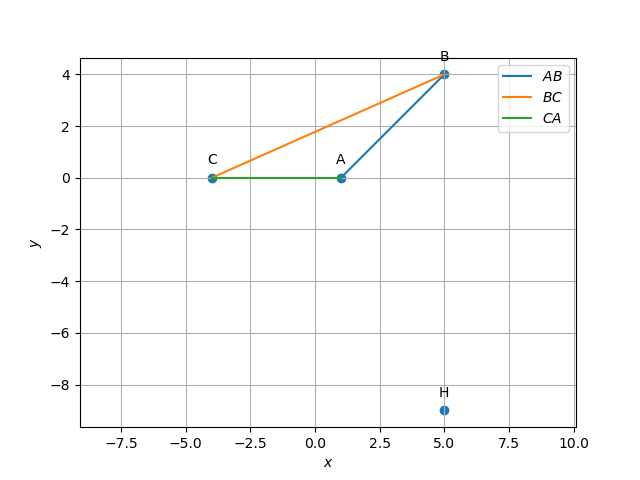
\includegraphics{/sdcard/digital-design/figs/orthocentre1.png}
    \caption{Ortho centre of $\triangle$ ABC}
    \label{fig:mat_alt1}
\end{figure}


\subsection{Perpendicular Bisector}

  
\begin{enumerate}[label=\thesubsection.\arabic*.,ref=\thesubsection.\theenumi]
\numberwithin{equation}{enumi}
%Question 1.6.4.1
\item Find the normal matrix for the perpendicular bisectors \\
\solution The normal matrix is $\vec{M}_2$
\begin{align}
       \vec{M}_2 &=\myvec{9 & -5 & -4 \\ 4 & 0 & -4}
\end{align}
\begin{figure}[H]
    \centering
    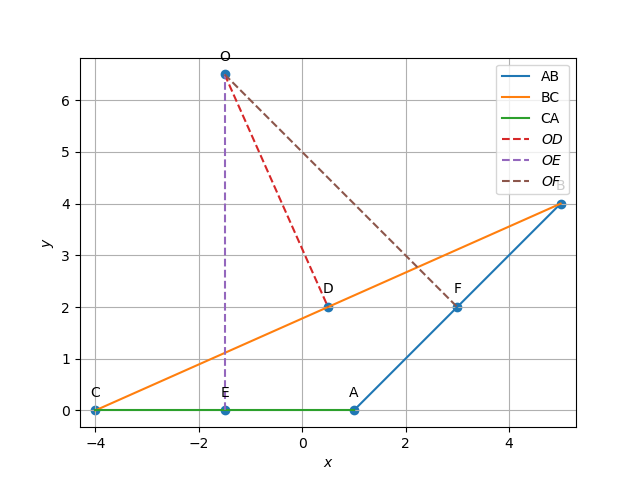
\includegraphics{/sdcard/digital-design/figs/pict1.png}
    \caption{plot of perpendicular bisectors}
    \label{fig:mat_perp1}
\end{figure}
%Question 1.6.4.2
\item Find the constants vector for the perpendicular bisectors. \\
\solution The desired vector is 
\begin{align}
\vec{c}_3 = \text{diag}\cbrak{\vec{M}_2^{\top}\myvec{\vec{D} & \vec{E} &\vec{F}}}
\end{align}
\solution
\begin{align}
\vec{c}_3 &= \text{diag}\cbrak{\vec{M}_2^{\top}\myvec{\vec{D} & \vec{E} &\vec{F}}} \\
\vec{M}_2^{\top}\myvec{\vec{D} & \vec{E} &\vec{F}} &= \myvec{9&4 \\ -5&0 \\ -4 &-4}\myvec{\frac{1}{2} & \frac{-3}{2} & 3 \\ 2 & 0 & 2} \\
\end{align}
Using matrix multiplication
\begin{align}
 \vec{M}_2^{\top}\myvec{\vec{D} & \vec{E} &\vec{F}} &=\myvec{ \frac{25}{2} & \frac{-27}{2} & 35 \\ \frac{-5}{2} & \frac{15}{2} & -15 \\ -10 & 6 & -20 } \\
    \vec{c}_3 &= \text{diag}\brak{ \myvec{ \frac{25}{2} & \frac{-27}{2} & 35 \\ \frac{-5}{2} & \frac{15}{2} & -15 \\ -10 & 6 & -20 }   } \\
 \vec{c}_3   &= \myvec{ \frac{25}{2} & \frac{15}{2} & -20}
\end{align}
\begin{figure}[H]
    \centering
    \includegraphics{/sdcard/digital-design/perp-bisect.png}
    \caption{circumcentre and circumcircle of $\triangle$ ABC}
    \label{fig:mat_perp2}
\end{figure}
\end{enumerate}


\subsection{Angle Bisector}


\begin{enumerate}[label=\thesubsection.\arabic*.,ref=\thesubsection.\theenumi]
\numberwithin{equation}{enumi}
%Question 1.6.5.1
\item Find the points of contact. \\ 
\solution The points of contact are given by 
\begin{align}
\myvec{			\frac{n\vec{A}+p\vec{C}}{n+p}
&
\frac{p\vec{B}+m\vec{A}}{p+m}
&
\frac{m\vec{C}+n\vec{B}}{m+n}
}
= 	\myvec{\vec{A} & \vec{B} &\vec{C}}\myvec{\frac{n}{b} & \frac{m}{c} & 0\\0 & \frac{p}{c} & \frac{n}{a} \\\frac{p}{b} & 0 & \frac{m}{a}}
\end{align}
\begin{align}
    \myvec{\vec{p} & \vec{m} & \vec{n} } &=\frac{1}{2} \myvec{\vec{a} & \vec{b} & \vec{c}} \myvec{ -1 & 1 & 1 \\1 & -1 & 1 \\1 & 1 & -1 } \\
   &= \frac{1}{2}\myvec{ \sqrt{97}&  \sqrt{25} & \sqrt{32} }\myvec{ -1 & 1 & 1 \\1 & -1 & 1 \\1 & 1 & -1 }  \\
   &= \frac{1}{2}\myvec{ 9.848857802&  5 & 5.65684549 }\myvec{ -1 & 1 & 1 \\1 & -1 & 1 \\1 & 1 & -1 }
\end{align}
Using matrix multiplication 
\begin{align}
        \myvec{\vec{p} & \vec{m} & \vec{n} } &= \myvec{  0.403993844& 5.252851646 & 4.596006156 }   \\
\myvec{\vec{A} & \vec{B} &\vec{C}}\myvec{\frac{n}{b} & \frac{m}{c} & 0\\0 & \frac{p}{c} & \frac{n}{a} \\\frac{p}{b} & 0 & \frac{m}{a}} 
  &= \myvec{1 & 5 & -4 \\ 0 & 4 & 0} \myvec{\frac{4.596006156}{\sqrt{25}} & \frac{5.252851646}{\sqrt{32}} & 0\\0 & \frac{0.403993844}{\sqrt{32}} & \frac{4.596006156}{\sqrt{97}} \\\frac{0.403993844}{\sqrt{25}} & 0 & \frac{5.252851646}{\sqrt{97}}}
\end{align}
Using matrix multiplication We get the points of contact 
\begin{align}
    &= \myvec{ 0.596006156 & 1.28566722899 & 0.1998835027956 \\ 0 & 0.28566722899833 & 1.8666148901313 }
\end{align}
\begin{figure}[H]
    \centering
    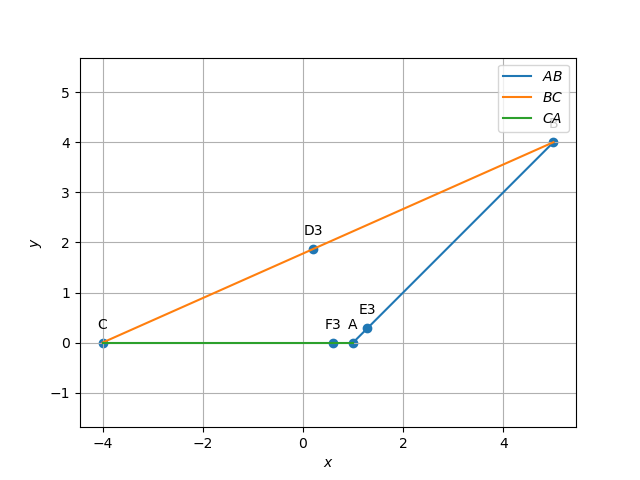
\includegraphics{/sdcard/digital-design/geometry/figs/points.png}
    \caption{Contact points of incircle of $triangle$ ABC}
    \label{fig:mat_ang1}
\end{figure}
\begin{figure}[H]
    \centering
    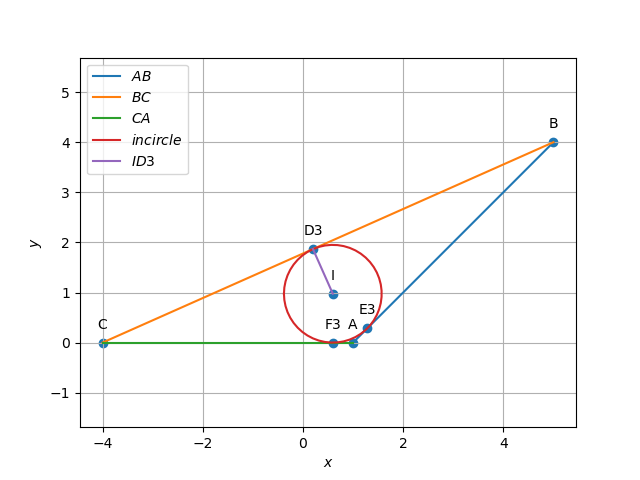
\includegraphics{/sdcard/digital-design/geometry/figs/incircle.png}
    \caption{Incircle and Incentre of $\triangle$ ABC }
    \label{fig:mat_ang2}
\end{figure}
\end{enumerate}


\end{document}
